\chapter{Конструкторский раздел}

%В данном разделе будет проведена формализация сущностей проектируемой системы, описаны используемые домены, ролевая модель и реализуемая табличная функция.

\section{Схема программного обеспечения}

На рисунке \ref{img:idef0} представлена IDEF0-диаграмма нулевого уровня разрабатываемого программно-аппаратного комплекса.

\begin{table}[h!]
  \centering
  \begin{tabular}{p{1\linewidth}}
    \centering
    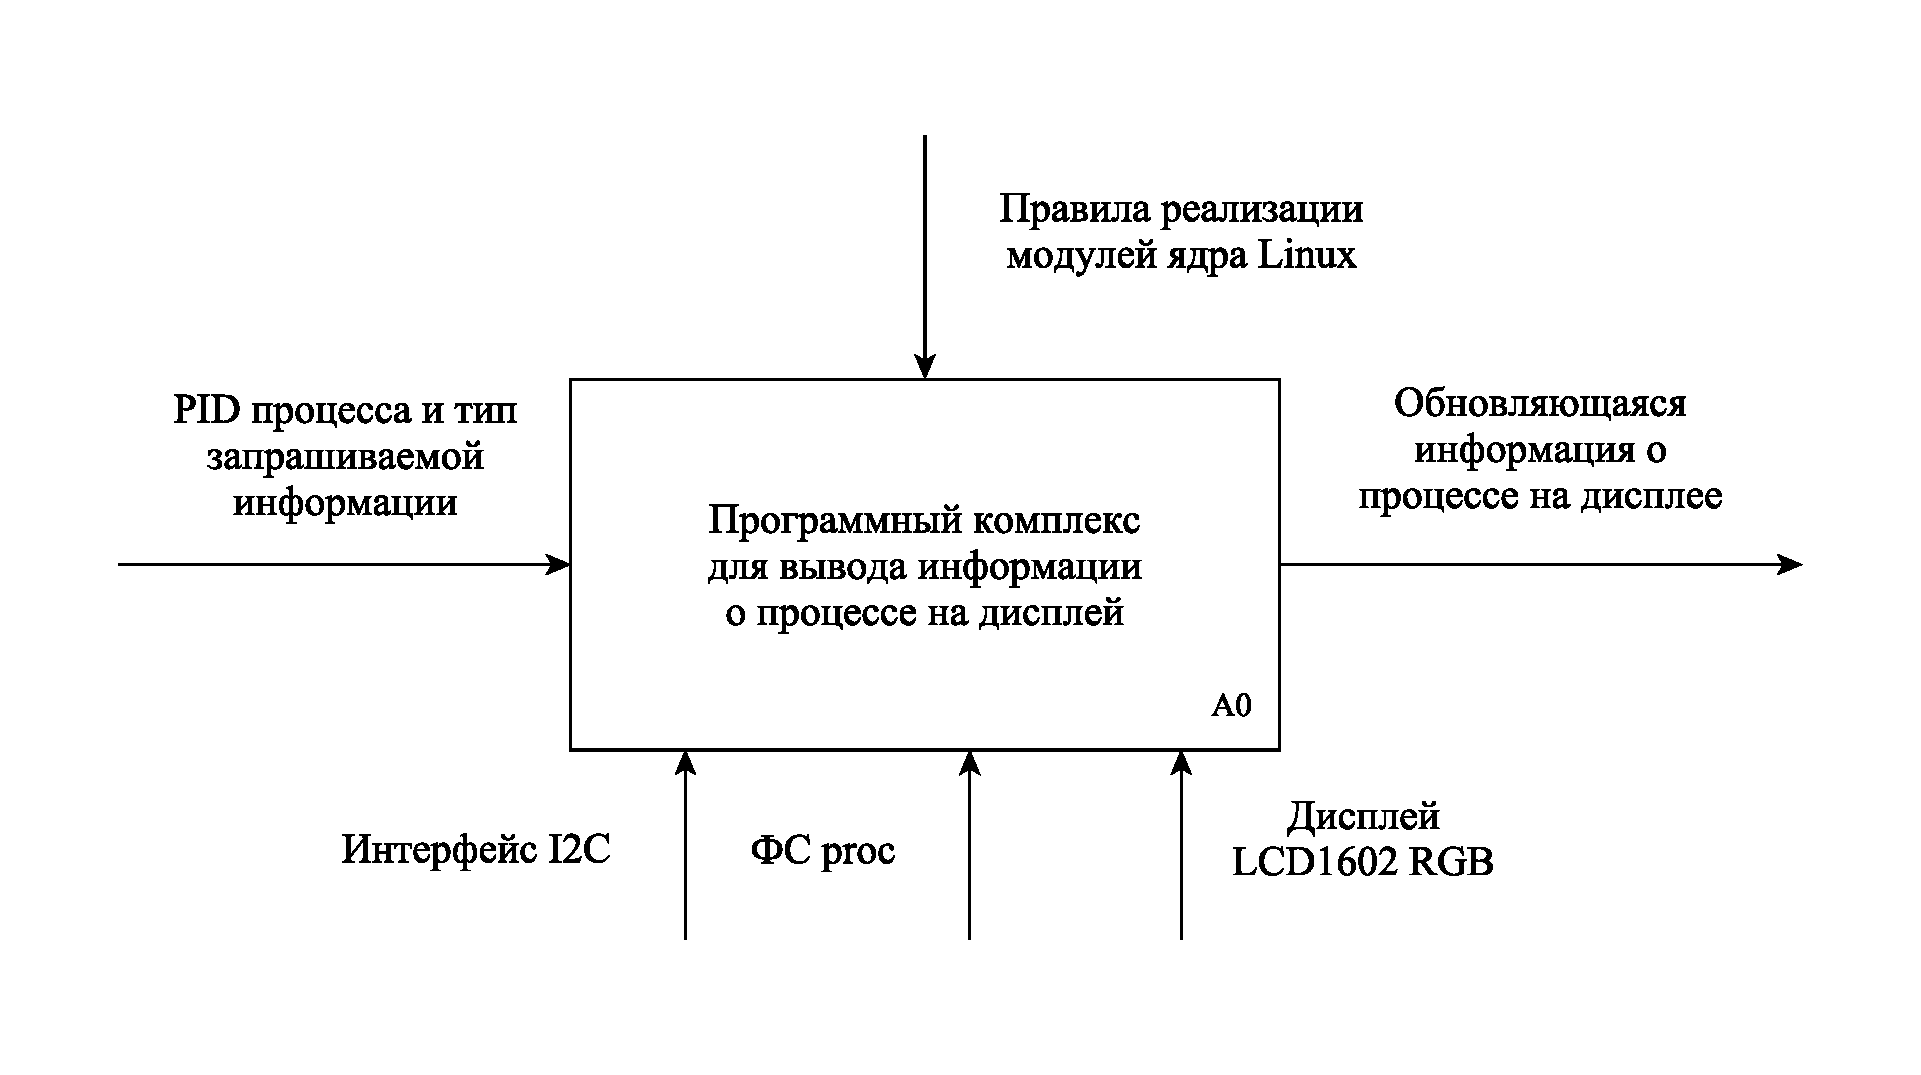
\includegraphics[width=1\linewidth]{./images/idef0.pdf}
    \captionof{figure}{IDEF0-диаграмма нулевого уровня разрабатываемого программно-аппаратного комплекса}
    \label{img:idef0}
  \end{tabular}
\end{table}

На рисунке \ref{img:idef1} представлена IDEF0-диаграмма первого уровня разрабатываемого программно-аппаратного комплекса.

\newpage

\begin{table}[h!]
  \centering
  \begin{tabular}{p{1\linewidth}}
    \centering
    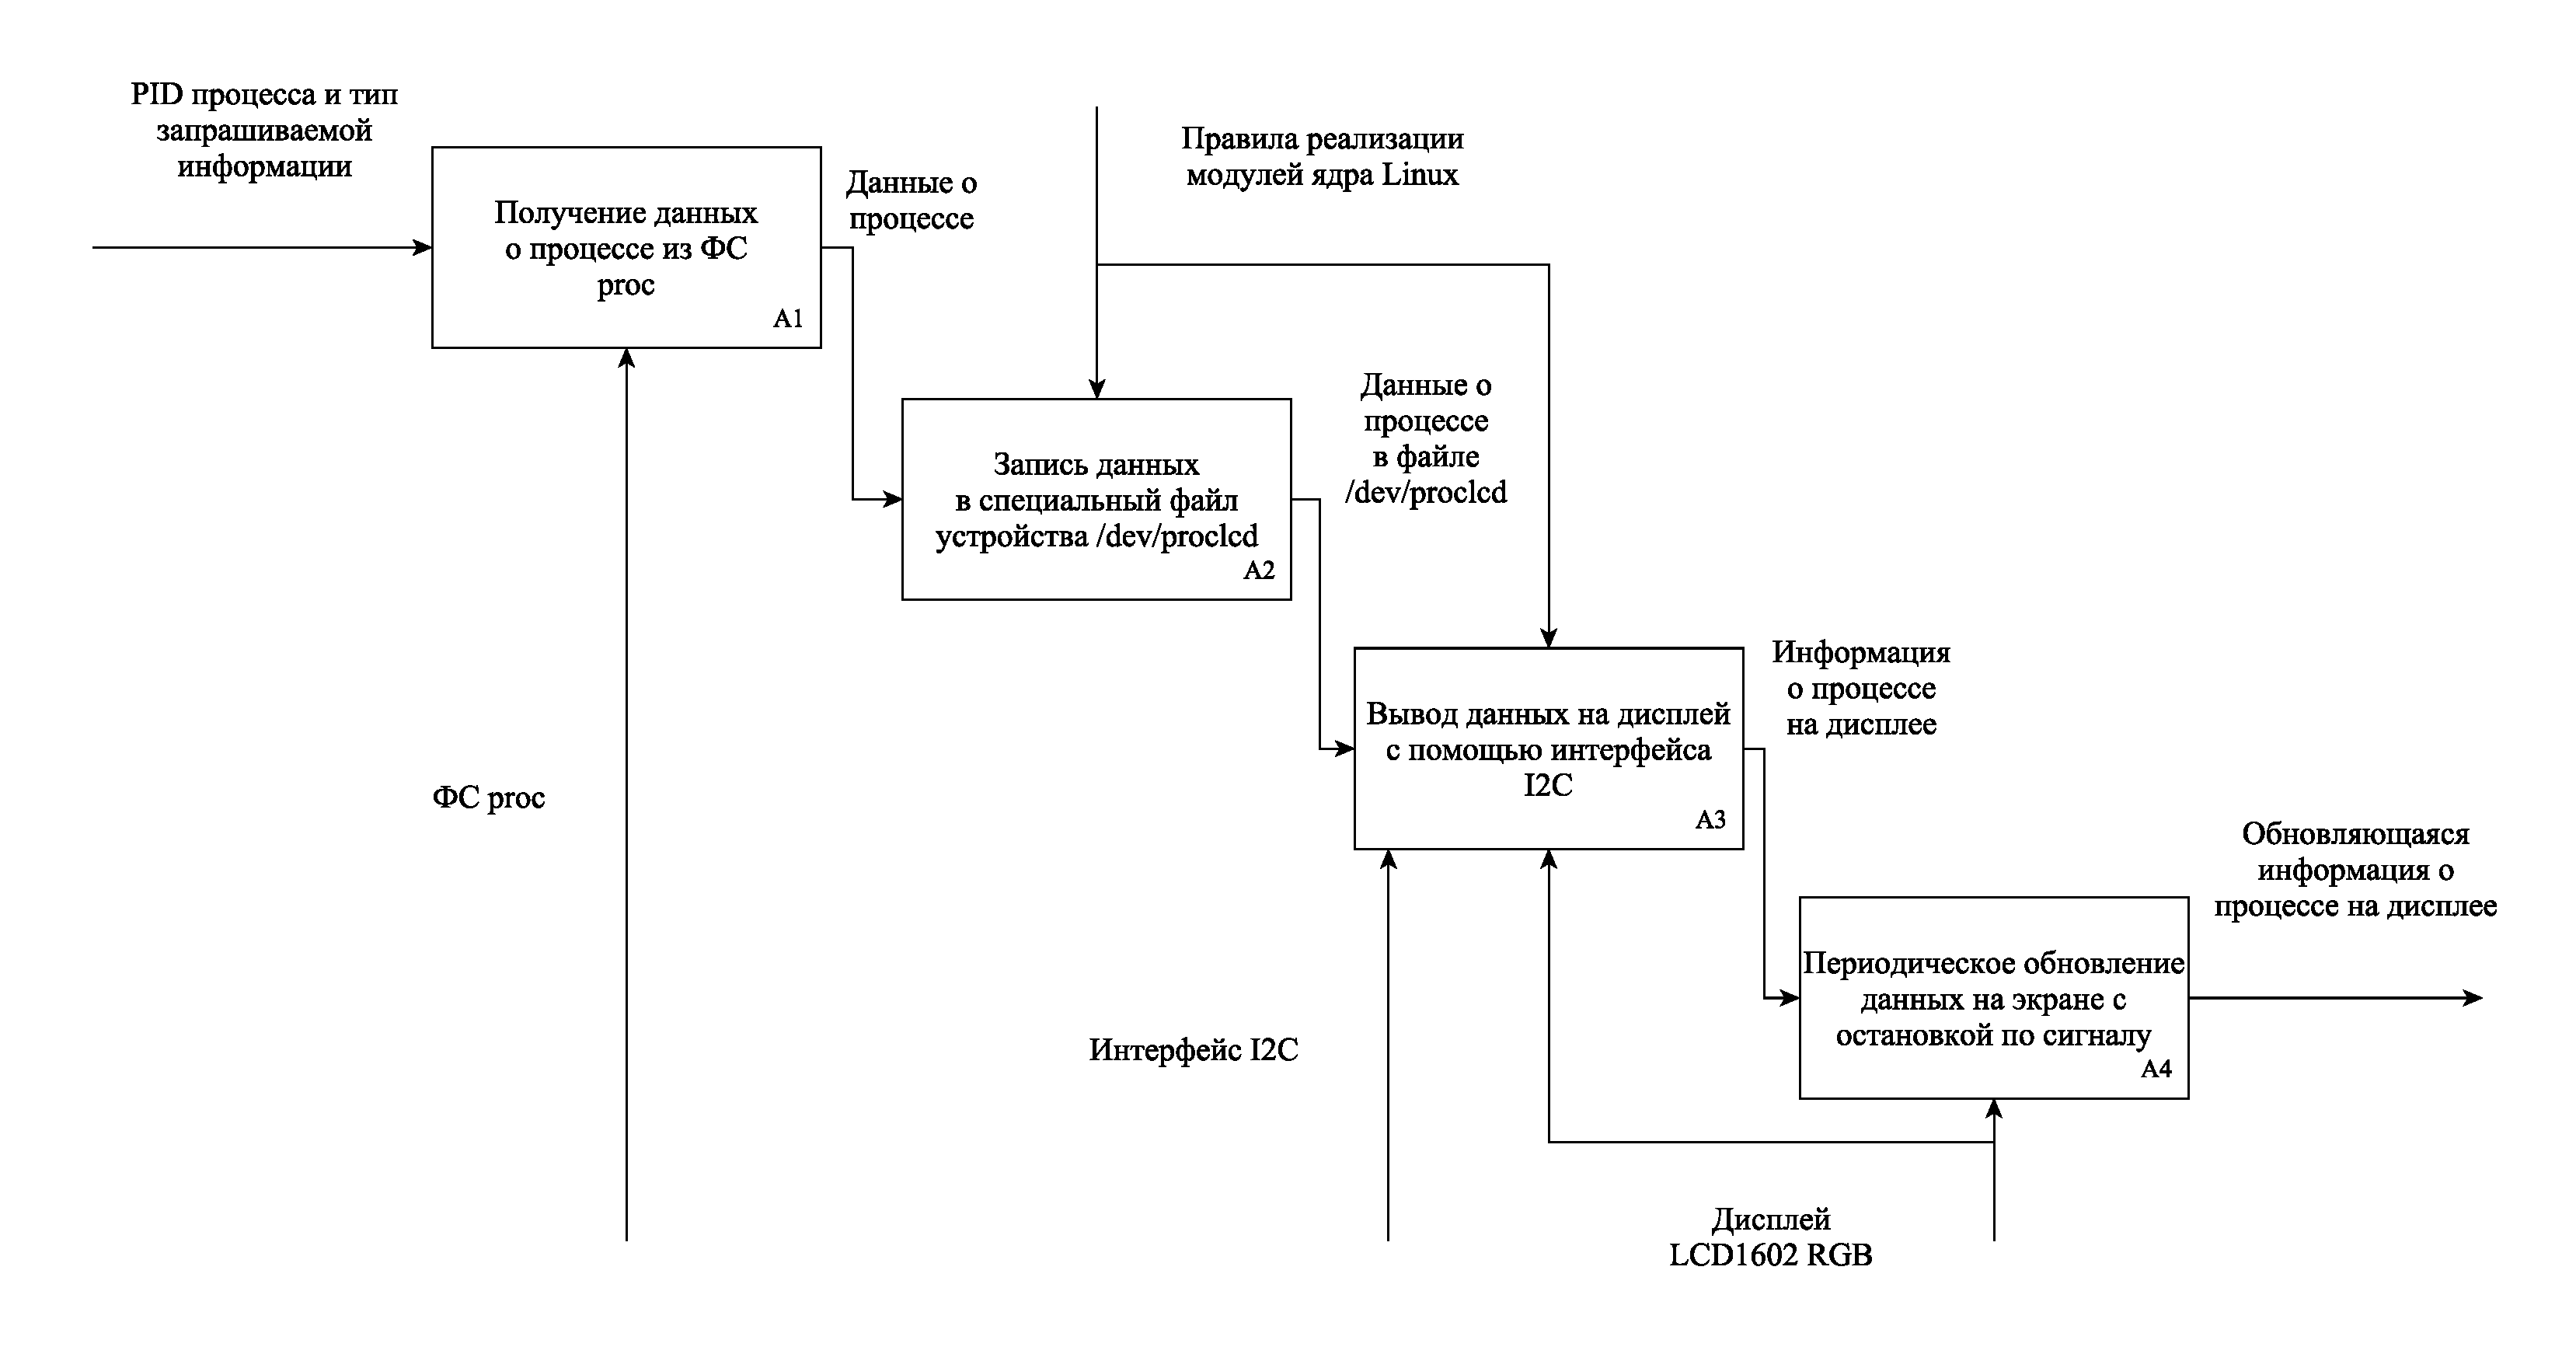
\includegraphics[width=1\linewidth]{./images/idef1.pdf}
    \captionof{figure}{IDEF0-диаграмма первого уровня разрабатываемого программно-аппаратного комплекса}
    \label{img:idef1}
  \end{tabular}
\end{table}

\newpage

\section{Схема алгоритма инициализации модуля ядра Linux~---~драйвера символьного дисплея}
На рисунке \ref{img:init} представлена схема алгоритма инициализации модуля ядра Linux~---~драйвера символьного дисплея.

\begin{table}[h!]
  \centering
  \begin{tabular}{p{1\linewidth}}
    \centering
    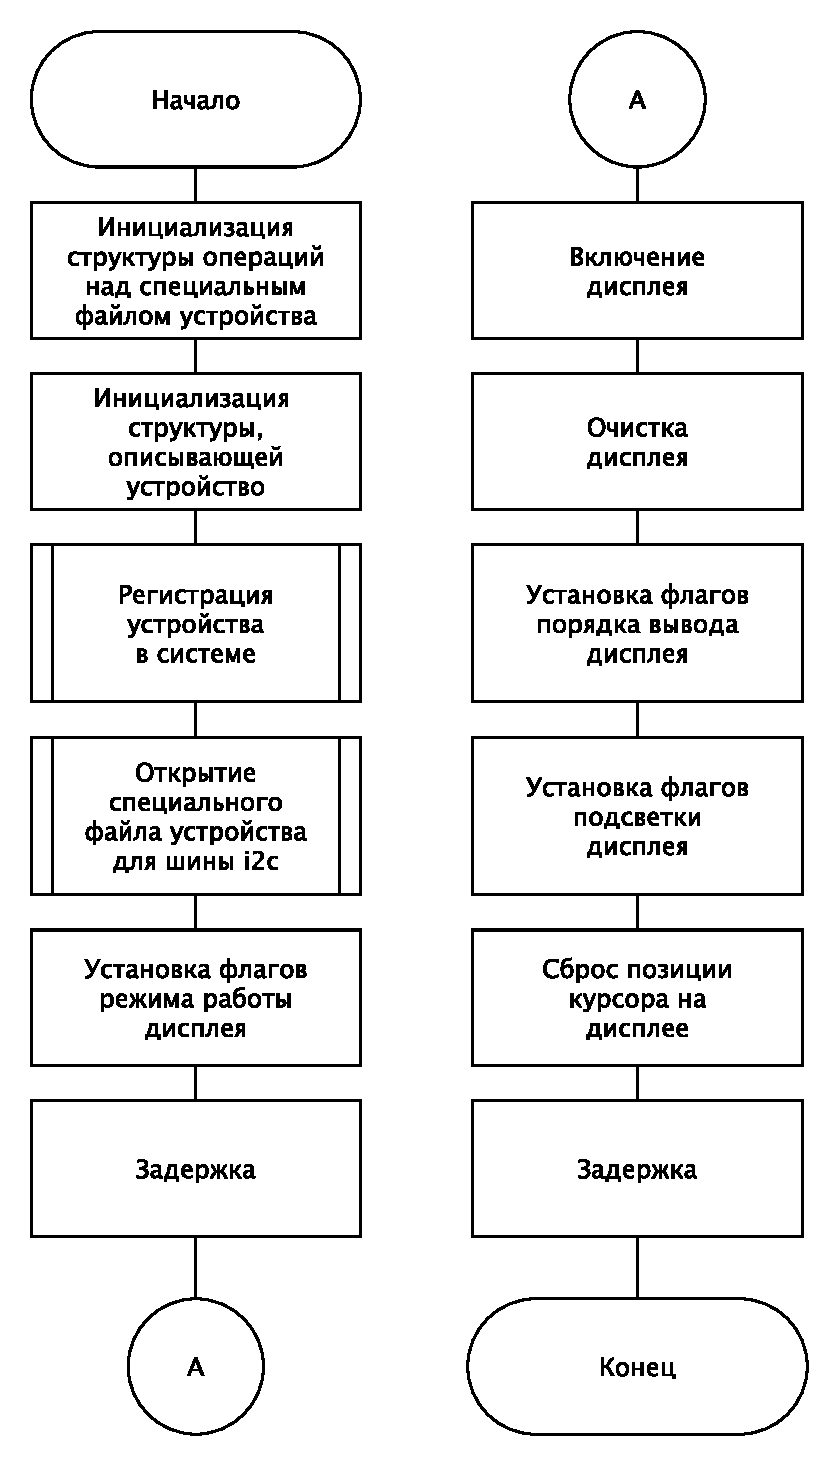
\includegraphics[width=0.65\linewidth]{./images/init.pdf}
    \captionof{figure}{Схема алгоритма инициализации модуля ядра Linux~---~драйвера символьного дисплея}
    \label{img:init}
  \end{tabular}
\end{table}

\newpage

\section{Схема алгоритма вывода данных на символьный дисплей}
На рисунке \ref{img:out} представлена схема алгоритма вывода данных на символьный дисплей.

\begin{table}[h!]
  \centering
  \begin{tabular}{p{1\linewidth}}
    \centering
    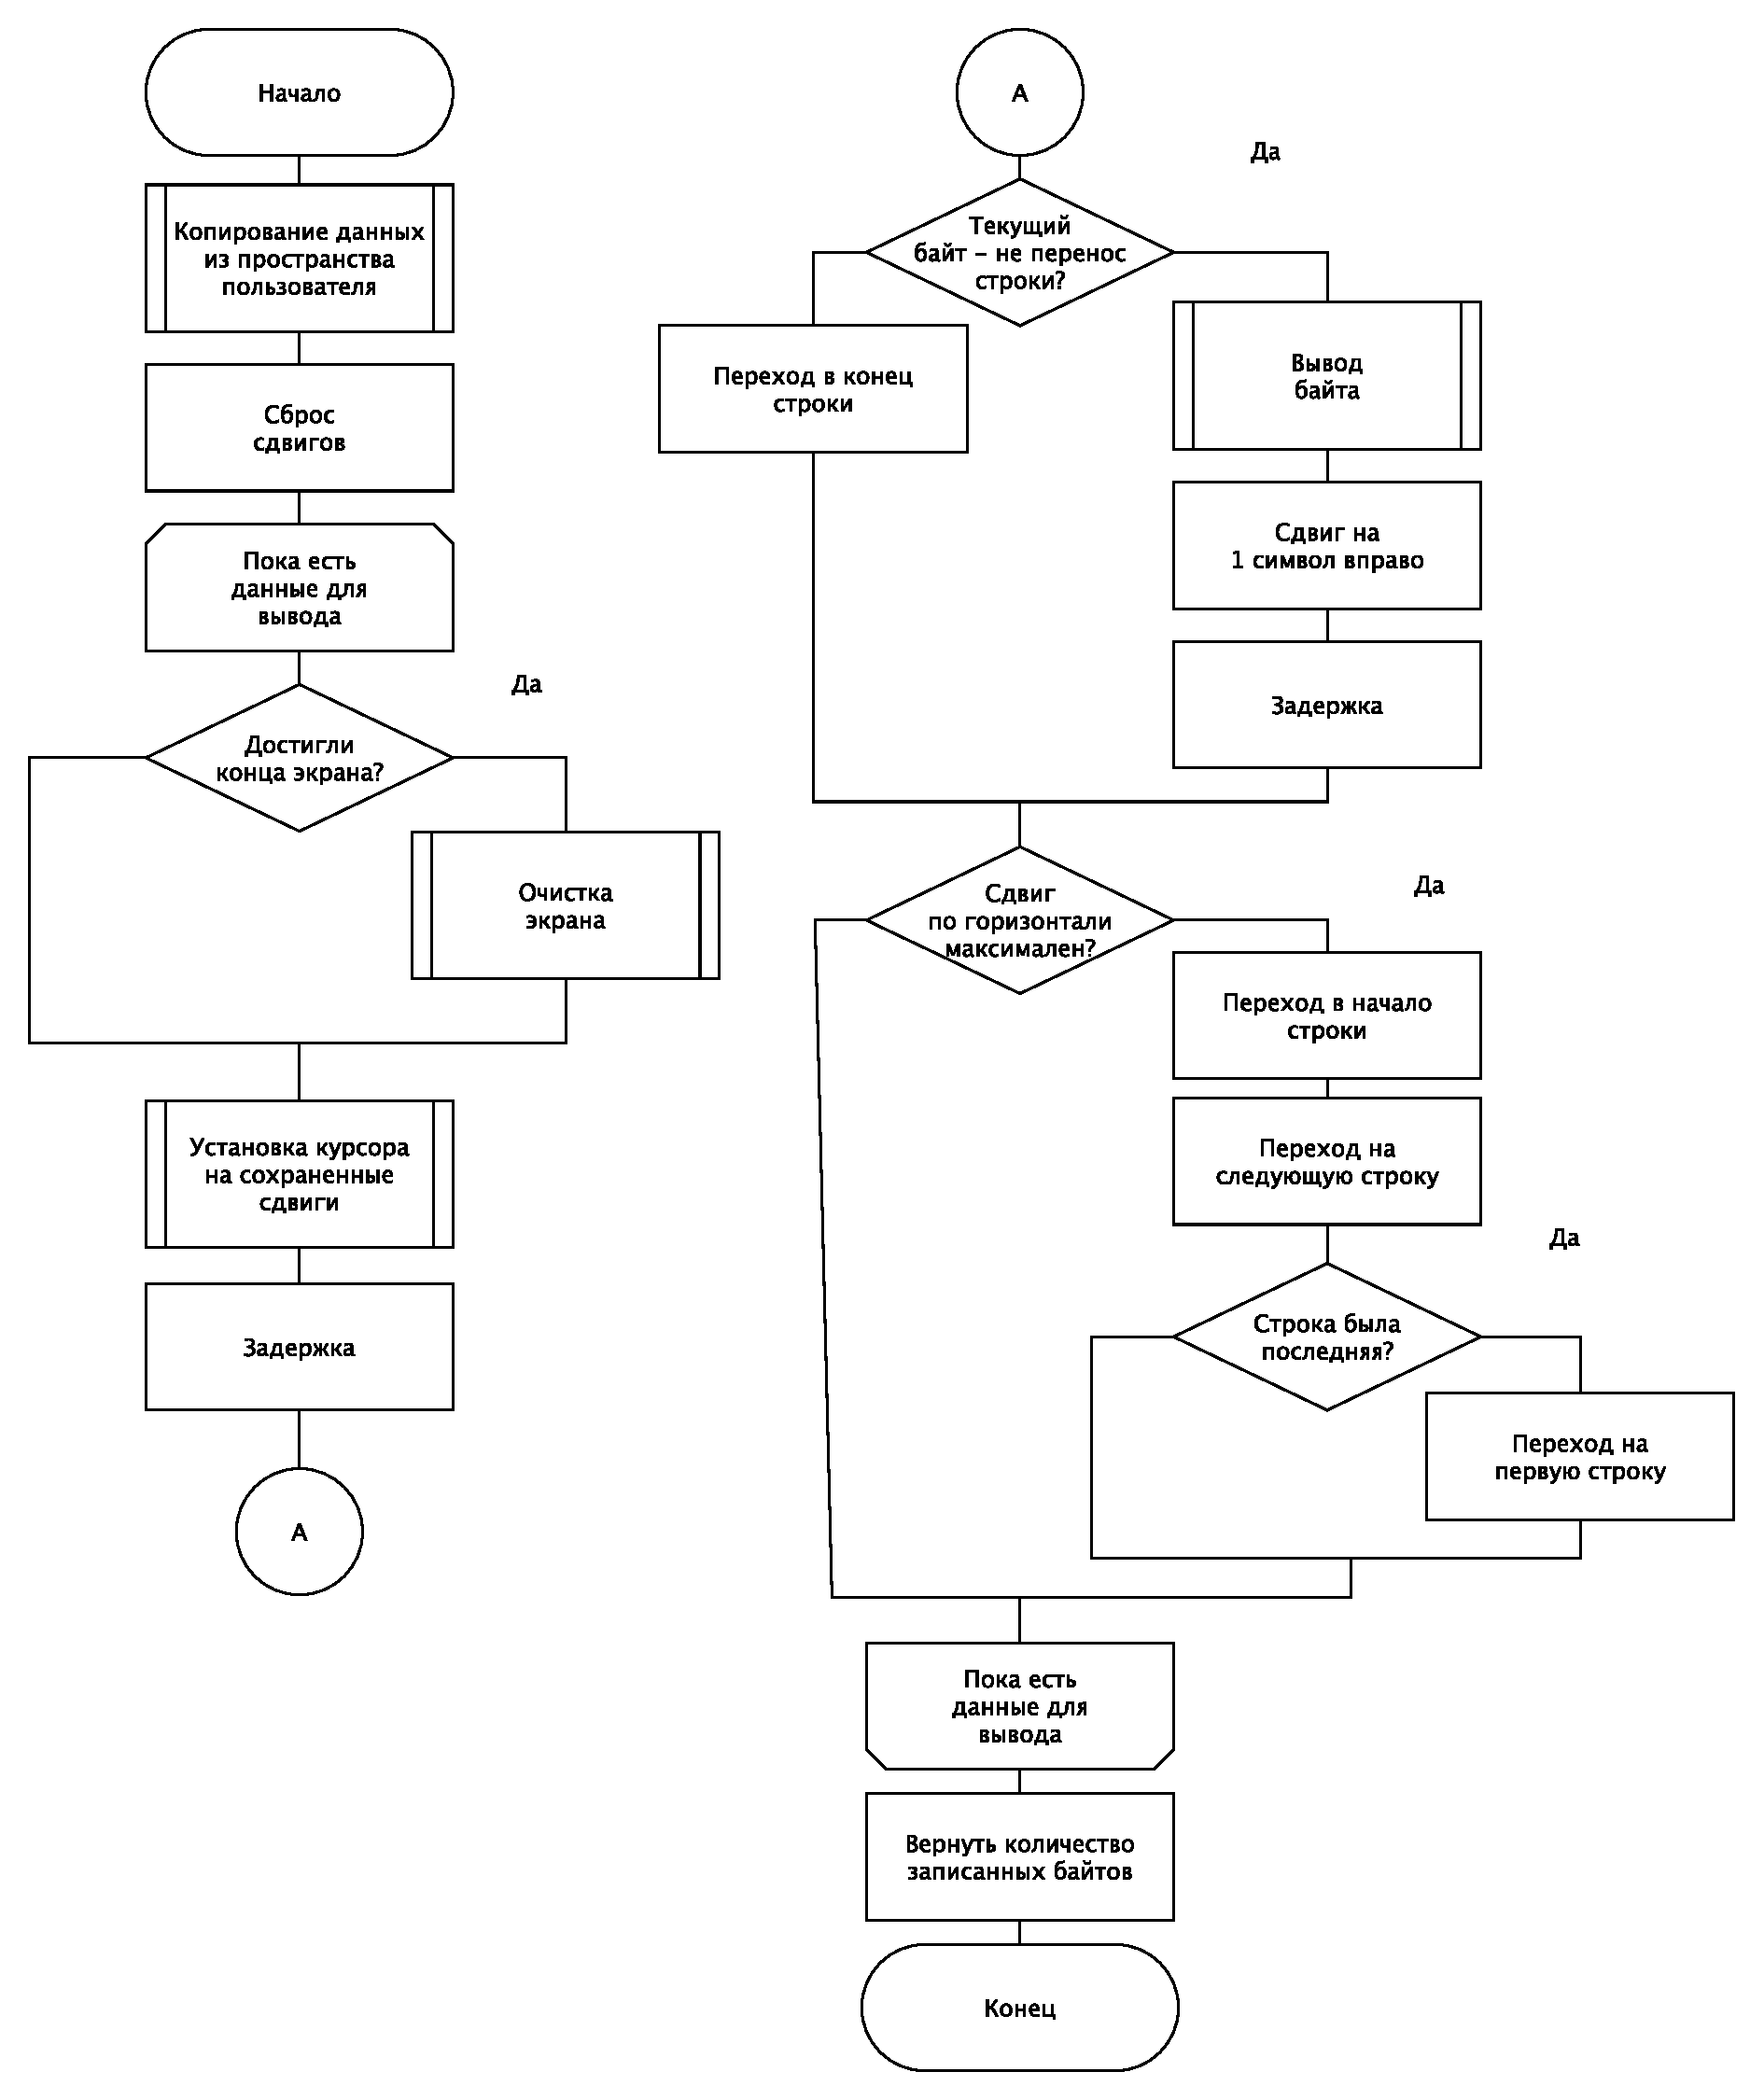
\includegraphics[width=0.98\linewidth]{./images/out.pdf}
    \captionof{figure}{Схема алгоритма вывода данных на символьный дисплей}
    \label{img:out}
  \end{tabular}
\end{table}

\newpage

\section{Схема алгоритма чтения данных из устройства}
На рисунке \ref{img:read} представлена схема алгоритма чтения данных из устройства.

\begin{table}[h!]
  \centering
  \begin{tabular}{p{1\linewidth}}
    \centering
    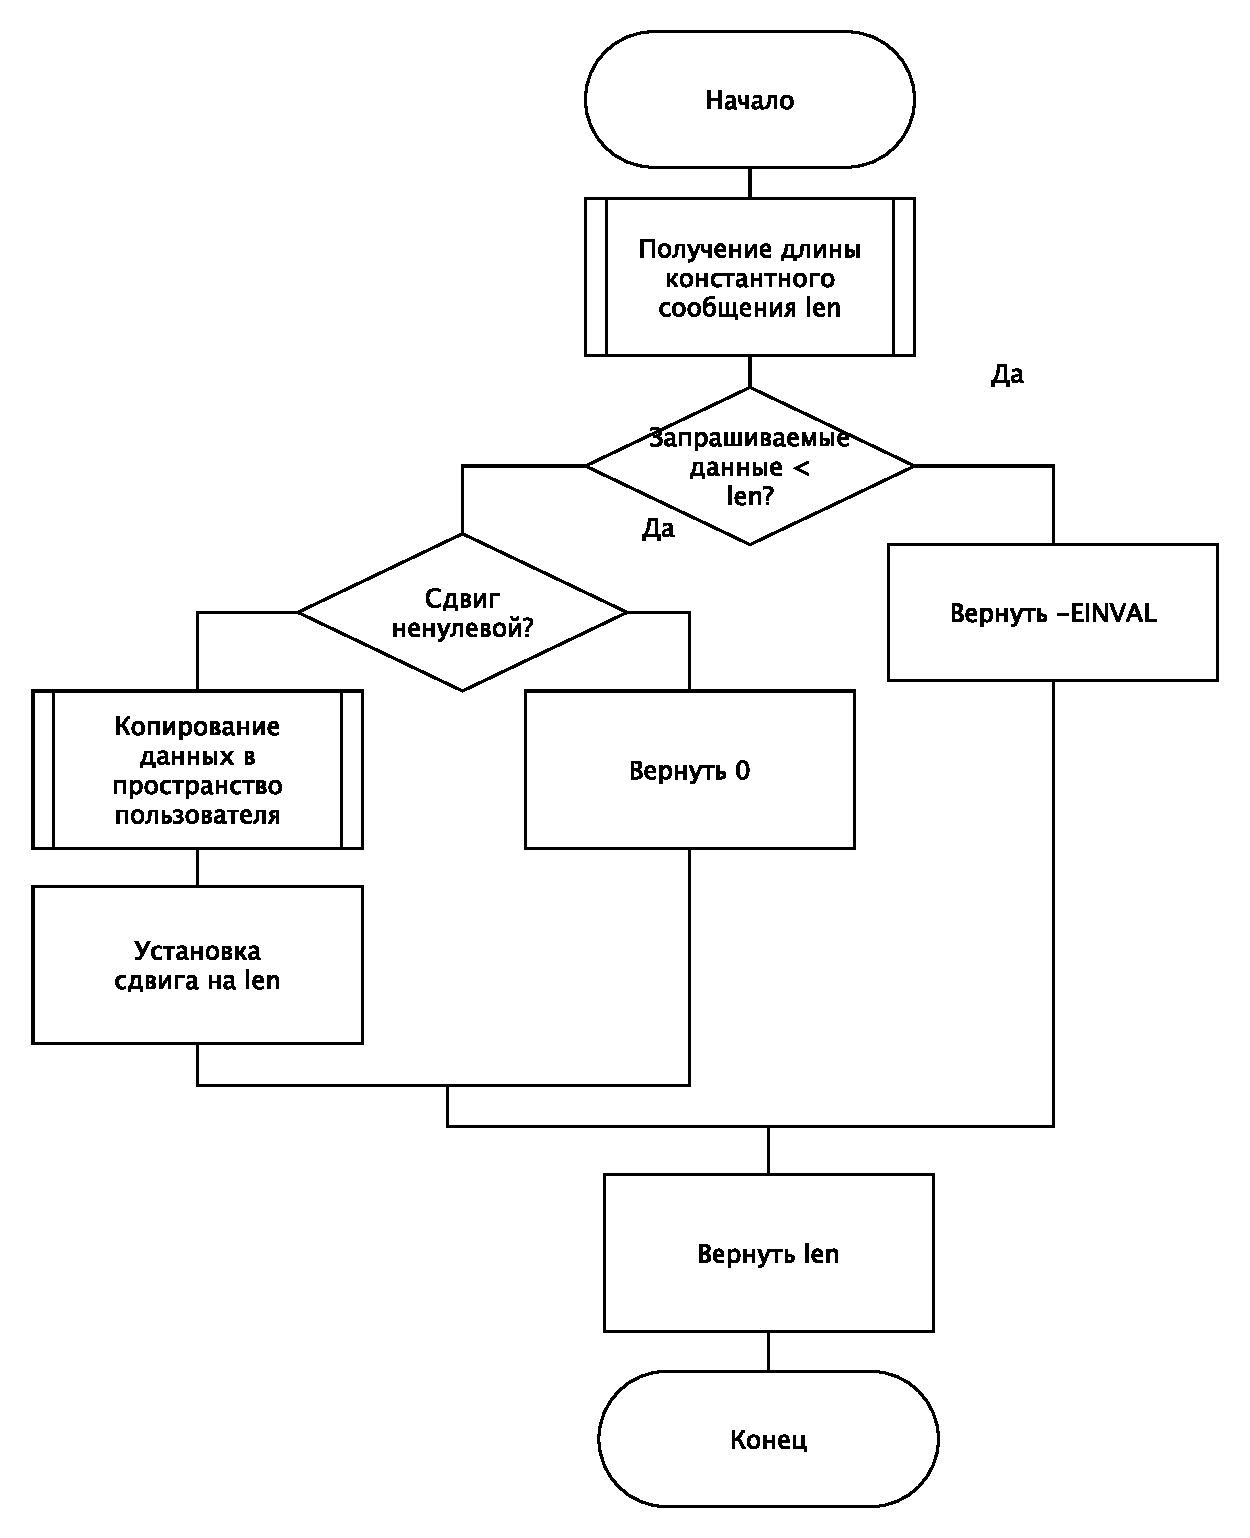
\includegraphics[width=0.9\linewidth]{./images/read.pdf}
    \captionof{figure}{Схема алгоритма чтения данных из устройства}
    \label{img:read}
  \end{tabular}
\end{table}

\newpage

\section{Схема алгоритма записи данных в шину через интерфейс I2C}

На рисунке \ref{img:write} представлена схема алгоритма записи данных в шину через интерфейс I2C.

\begin{table}[h!]
  \centering
  \begin{tabular}{p{1\linewidth}}
    \centering
    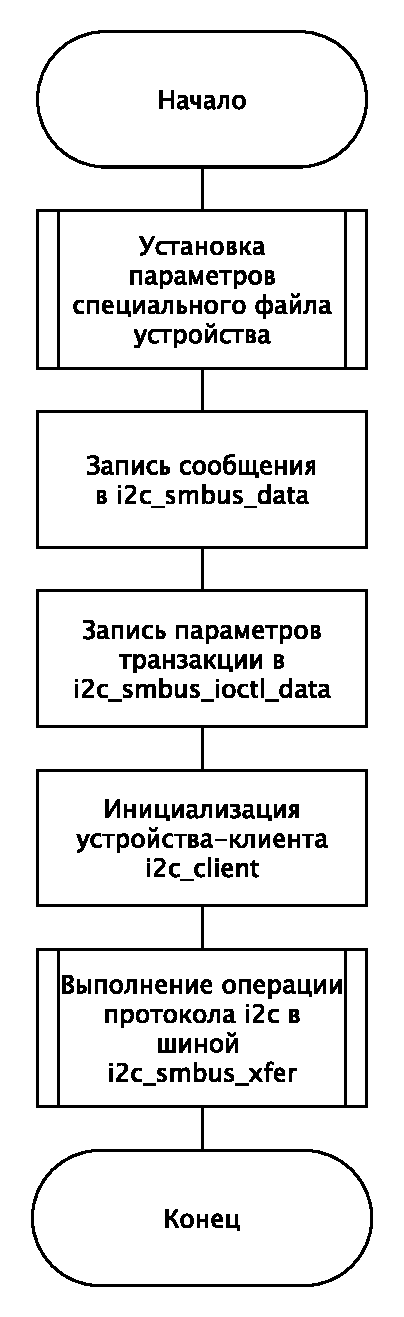
\includegraphics[width=0.35\linewidth]{./images/write.pdf}
    \captionof{figure}{Схема алгоритма записи данных в шину через интерфейс I2C}
    \label{img:write}
  \end{tabular}
\end{table}

\newpage

\section{Схема алгоритма работы клиентского приложения}
На рисунке \ref{img:client} представлена схема алгоритма работы клиентского приложения.

\begin{table}[h!]
  \centering
  \begin{tabular}{p{1\linewidth}}
    \centering
    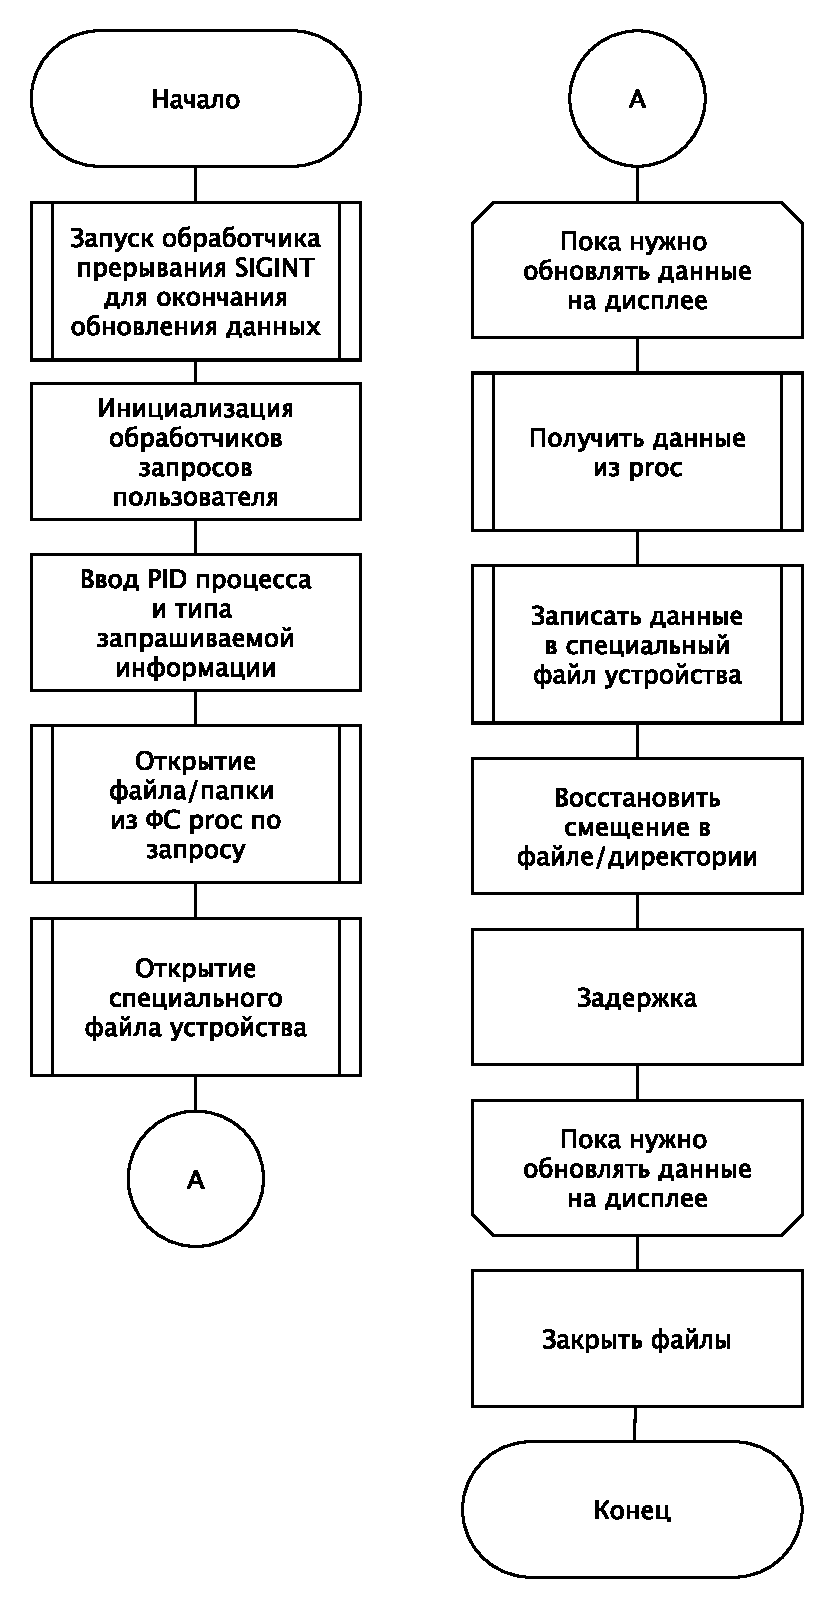
\includegraphics[width=0.6\linewidth]{./images/client.pdf}
    \captionof{figure}{Схема алгоритма работы клиентского приложения}
    \label{img:client}
  \end{tabular}
\end{table}

\section{Структуры ядра}

\subsection{struct file\_operations}

struct file\_operations~---~структура, содержащая либо стандартные операции на файлах для конкретной файловой системы, либо зарегистрированные разработчиком.

\begin{lstlisting}[label=struct_file_operations,caption=struct file\_operations]
struct file_operations {
	struct module *owner;
	loff_t (*llseek) (struct file *, loff_t, int);
	ssize_t (*read) (struct file *, char __user *, size_t, loff_t *);
	ssize_t (*write) (struct file *, const char __user *, size_t, loff_t *);
	...
	int (*open) (struct inode *, struct file *);
	int (*flush) (struct file *, fl_owner_t id);
	int (*release) (struct inode *, struct file *);
	...
} __randomize_layout;
\end{lstlisting}

\subsection{struct device}

struct device~---~базовая структура устройства, редко используется в чистом виде. parent~---~устройство, к которому подсоединено данное устройство, init\_name~---~имя устройства, type~---~тип устройства, bus~---~тип шины.

\begin{lstlisting}[label=struct_device,caption=struct device]
struct device {
	...
	struct device		*parent;
	...
	const char		*init_name; /* initial name of the device */
	const struct device_type *type;

	struct bus_type	*bus;		/* type of bus device is on */
	struct device_driver *driver;	/* which driver has allocated this
					   device */
	void		*platform_data;	/* Platform specific data, device
					   core doesn't touch it */
	void		*driver_data;	/* Driver data, set and get with
					   dev_set_drvdata/dev_get_drvdata */
	struct mutex		mutex;	/* mutex to synchronize calls to
					 * its driver.
					 */
	...
};
\end{lstlisting}

\subsection{struct miscdevice}

struct miscdevice~---~структура, описывающая устройство. Используется при реализации небольших драйверов и является упрощённой по сравнению с struct cdev~\cite{bib8}. Система хранит все старшие номера устройств в статической таблице, поэтому выделение старших номеров под простые драйверы считается излишним. Устройства, зарегистрированные, как miscdevice, получают старший номер равный 10. Также, при использовании miscdevice, специальный файл устройства создается сразу при регистрации устройства, а при выборе cdev его нужно создавать отдельно.

\begin{lstlisting}[label=struct_miscdevice,caption=struct miscdevice]
struct miscdevice  {
	int minor;
	const char *name;
	const struct file_operations *fops;
	struct list_head list;
	struct device *parent;
	struct device *this_device;
	const struct attribute_group **groups;
	const char *nodename;
	umode_t mode;
};
\end{lstlisting}

\subsection{struct file}

struct file~---~структура, которая описывает открытый файл.

\begin{lstlisting}[label=struct_file,caption=struct file]
struct file {
	...
	struct path		f_path;
	struct inode		*f_inode;	/* cached value */
	const struct file_operations	*f_op;
	...
	atomic_long_t		f_count;
	unsigned int 		f_flags;
	fmode_t			f_mode;
	struct mutex		f_pos_lock;
	loff_t			f_pos;
	...
	struct address_space	*f_mapping;
	...
} __randomize_layout
  __attribute__((aligned(4)));
\end{lstlisting}

\subsection{union i2c\_smbus\_data}

union i2c\_smbus\_data~---~сообщение, передаваемое по шине I2C.

\begin{lstlisting}[label=union_i2c_smbus_data,caption=union i2c\_smbus\_data]
#define I2C_SMBUS_BLOCK_MAX	32	/* As specified in SMBus standard */
union i2c_smbus_data {
	__u8 byte;
	__u16 word;
	__u8 block[I2C_SMBUS_BLOCK_MAX + 2]; /* block[0] is used for length */
			       /* and one more for user-space compatibility */
};
\end{lstlisting}

\subsection{struct i2c\_smbus\_ioctl\_data}

struct i2c\_smbus\_ioctl\_data~---~структура, использующаяся в вызове ioctl.

\begin{lstlisting}[label=struct_i2c_smbus_ioctl_data,caption=struct i2c\_smbus\_ioctl\_data]
/* This is the structure as used in the I2C_SMBUS ioctl call */
struct i2c_smbus_ioctl_data {
	__u8 read_write;
	__u8 command;
	__u32 size;
	union i2c_smbus_data __user *data;
};
\end{lstlisting}

\subsection{struct i2c\_client}

struct i2c\_client представляет ведомое устройство I2C, подключенное к шине. addr~---~адрес на I2C шине, name~---~имя чипа устройства, идентифицирует тип устройства, dev~---~структура-описатель устройства, adapter~---~сегмент шины, к которому подключено устройство.

\begin{lstlisting}[label=struct_i2c_client,caption=struct i2c\_client]
struct i2c_client {
	unsigned short flags;		/* div., see below		*/
	unsigned short addr;		/* chip address - NOTE: 7bit	*/
					/* addresses are stored in the	*/
					/* _LOWER_ 7 bits		*/
	char name[I2C_NAME_SIZE];
	struct i2c_adapter *adapter;	/* the adapter we sit on	*/
	struct device dev;		/* the device structure		*/
	int init_irq;			/* irq set at initialization	*/
	int irq;			/* irq issued by device		*/
	struct list_head detected;
#if IS_ENABLED(CONFIG_I2C_SLAVE)
	i2c_slave_cb_t slave_cb;	/* callback for slave mode	*/
#endif
	void *devres_group_id;		/* ID of probe devres group	*/
};
\end{lstlisting}

\section{Точки входа драйвера}

Драйвер имеет следующие точки входа:

\begin{enumerate}
	\item \texttt{my\_init}~---~инициализация модуля;
	\item \texttt{my\_exit}~---~завершение работы модуля;
	\item \texttt{dev\_read}~---~чтение из специального файла устройства;
	\item \texttt{dev\_write}~---~запись в специальный файл устройства.
\end{enumerate}

\section{Взаимодействие модулей ПО}

На рисунке \ref{img:modules} представлена схема взаимодействия модулей ПО.

\newpage

\begin{table}[h!]
  \centering
  \begin{tabular}{p{1\linewidth}}
    \centering
    \includegraphics[width=0.98\linewidth]{./images/modules.pdf}
    \captionof{figure}{Схема взаимодействия модулей ПО}
    \label{img:modules}
  \end{tabular}
\end{table}

\section*{Вывод}
Были составлены схемы алгоритмов инициализации модуля ядра~---~драйвера символьного дисплея, вывода данных на символьный дисплей, чтения данных из устройства, записи данных в шину через интерфейс I2C и работы клиентского приложения. Были приведены необходимые для разработки структуры ядра, описаны точки входа драйвера символьного дисплея. Также, была представлена схема взаимодействия модулей программного комплекса.



